\documentclass[letterpaper,oneside]{scrartcl}
\usepackage{fullpage}
\usepackage[utf8]{inputenc}
\usepackage[pdftex]{graphicx}
\DeclareGraphicsExtensions{.png,.pdf}
\usepackage{hyperref}
\usepackage{color}
\definecolor{slateblue}{rgb}{0.07,0.07,0.488}
\hypersetup{colorlinks=true,linkcolor=slateblue,anchorcolor=slateblue,citecolor=slateblue,filecolor=slateblue,urlcolor=slateblue,bookmarksnumbered=true,pdfview=FitB}
\usepackage{url}
\usepackage[round,sectionbib]{natbib}
\bibliographystyle{abbrvnat}
\usepackage[small]{caption2}
\usepackage[small]{titlesec}
\renewcommand\familydefault{bch}
\usepackage{slashbox}
\usepackage{booktabs}

\title{plyr: divide and conquer}
\author{Hadley Wickham}
\begin{document}
\maketitle

% \begin{abstract}
% plyr is a set of tools that solves a common set of problems: you need to break a big problem down into manageable pieces, operate on each pieces and then put all the pieces back together.  This paper describes the components that make up plyr.  It includes two case studies.
% \end{abstract}

\section{Introduction}

The {\tt plyr} package provides tools for solving a common class of problems, where you break apart a big complicated data structure into small simple pieces, operate on each piece independently and then put all the pieces back together (possibly in a different format to the original).  This paper introduces the {\tt ply} family of functions which generalise the {\tt apply} family found in the base package, and include all combinations of input and output of lists, data frames and arrays.

This paper describes version 0.1 of {\tt plyr}, which requires R 2.7.0 or later and has no run-time dependencies.  To install it from within R, run {\tt install.packages("plyr")}.  Information about the latest version of the package can be found online at \url{http://had.co.nz/plyr}.  

% If you have any questions or comments about {\tt plyr}, please feel free to email me directly at \href{mailto:h.wickham@gmail.com}{h.wickham@gmail.com}.

In general, plyr provides a replacement for loops for a large set of practical problems.  The major assumption that the {\tt ply} functions make is that each piece can be operated on independently of the other pieces, so if there is any dependence between the pieces then you will need to use other tools.  The need to provide an alternative to loops does not come about because loops are slow (they are not!), but because they do not clearly express the intent of the algorithm, as important details are mixed in with unimportant book-keeping code. The tools of {\tt plyr} aim to eliminate this extra code and illuminate the key components of your computations.

Section~\ref{sec:usage} introduces the {\tt plyr} family of tools and how to use them.  The {\tt plyr} package also provides a number of helper functions for error recovery, splatting, column-wise processing, and reporting progress,  described in Section~\ref{sec:helpers}. Section~\ref{sec:strategy} discusses the general strategy that these functions support, including cases studies that explore the performance of veteran baseball players and ozone measured over space and time.  Finally, Section~\ref{sec:equiv} maps existing R functions to their plyr counterparts and lists related packages.  Section~\ref{sec:future} describes future plans.

\section{Usage}
\label{sec:usage}

Table~\ref{tbl:functions} lists the basic set of plyr functions.  Each function is named according to the type of input it accepts and the type of output it produces.  The input type determines how the big data structure can be broken down into small pieces, and the output type determines how the pieces are joined back together again.  Breaking down input is described in Section~\ref{sec:input} and piecing together output is described in Section~\ref{sec:output}.

{\bf NB}: In this paper, the term {\bf array} includes the special cases of vectors (1d arrays) and matrices (2d arrays) as well, and {\bf list-array} is used to refer to an array made out of a list (as opposed to an atomic vector, as is more usual).

\begin{table}
  \begin{center}
  \begin{tabular}{|l|ccc|}
    \hline
    \backslashbox{{\bf to}}{{\bf from}} & array & data frame & list \\
    \hline
    array      & aaply  & daply  & laply  \\
    data frame & adply  & ddply  & ldply  \\
    list       & alply  & dlply  & llply  \\
    nothing    & a\_ply & d\_ply & l\_ply \\
    \hline
  \end{tabular}
  \end{center}
  \caption{The 12 key functions that make up {\tt plyr}.  Arrays include matrices and vectors as special cases.}
  \label{tbl:functions}
\end{table}

Arguments to the ply functions are determined by the types of input and output.  For this reason, it's useful to refer to a complete row or column of Table~\ref{tbl:functions}.  The notation we use for this is {\tt d*ply} to refer an entire row (fixed input) and {\tt *dply} for an entire column (fixed output).

Plyr functions have either two or three main arguments, depending on the type of input:

\begin{itemize}
  \item {\tt a*ply(data., margins., fun., ..., progress. = "none")}
  \item {\tt d*ply(data., variables., fun., ..., progress. = "none")}
  \item {\tt l*ply(data., fun., ..., progress. = "none")}
\end{itemize}

The first argument is the {\tt data} to be split up, processed and recombined.  For arrays and data frames, the second argument describes how to split up the data by {\tt margins} or by {\tt variables}.  The third argument is the function to be applied to each piece.  All further arguments are passed on to the processing function.  The {\tt .progress} argument controls displaying of a progress bar, and is described at the end of Section~\ref{sec:helpers}.

Note that all {\tt plyr} arguments are suffixed with ``{\tt .}'' - this is to help prevent clashes with arguments in the processing function.  Recommended practice is to call {\tt **ply} functions with arguments specified by position, not name.

\subsection{Input} 
\label{sec:input}

\begin{itemize}
  \item Arrays are sliced 
  
  \item Data frames are split into groups based on combinations of variables
  
  \item Lists are assumed to be broken up already, and so this argument is omitted
  
\end{itemize}

\subsubsection{In: array ({\tt a*ply})}

The {\tt margins} argument of {\tt a*ply} describes how to slice up the array in the same way that {\tt apply} does.  For example, {\tt margins = 1} specifies that we want to break up the array by rows (the first index when subsetting), and {\tt margins = 2} by columns (the second index when subsetting).  You can also use combinations of margins.  For example, {\tt margins = 1:2} will split up by the first two dimensions.  For a 3d array, this will produce the columns in the z-direction.

\begin{figure}[htbp]
  \centering
    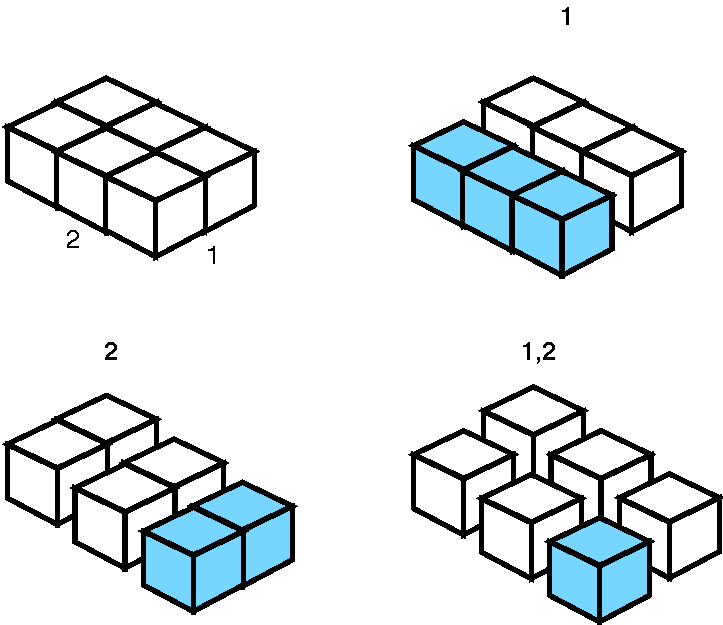
\includegraphics[width= 0.4 \textwidth]{split-matrix}
  \caption{The four ways to split up a 2d matrix.  Original matrix shown at top left.  Blue indicates a single piece of the output.}
  \label{fig:split-matrix}
\end{figure}
\begin{figure}[htbp]
  \centering
    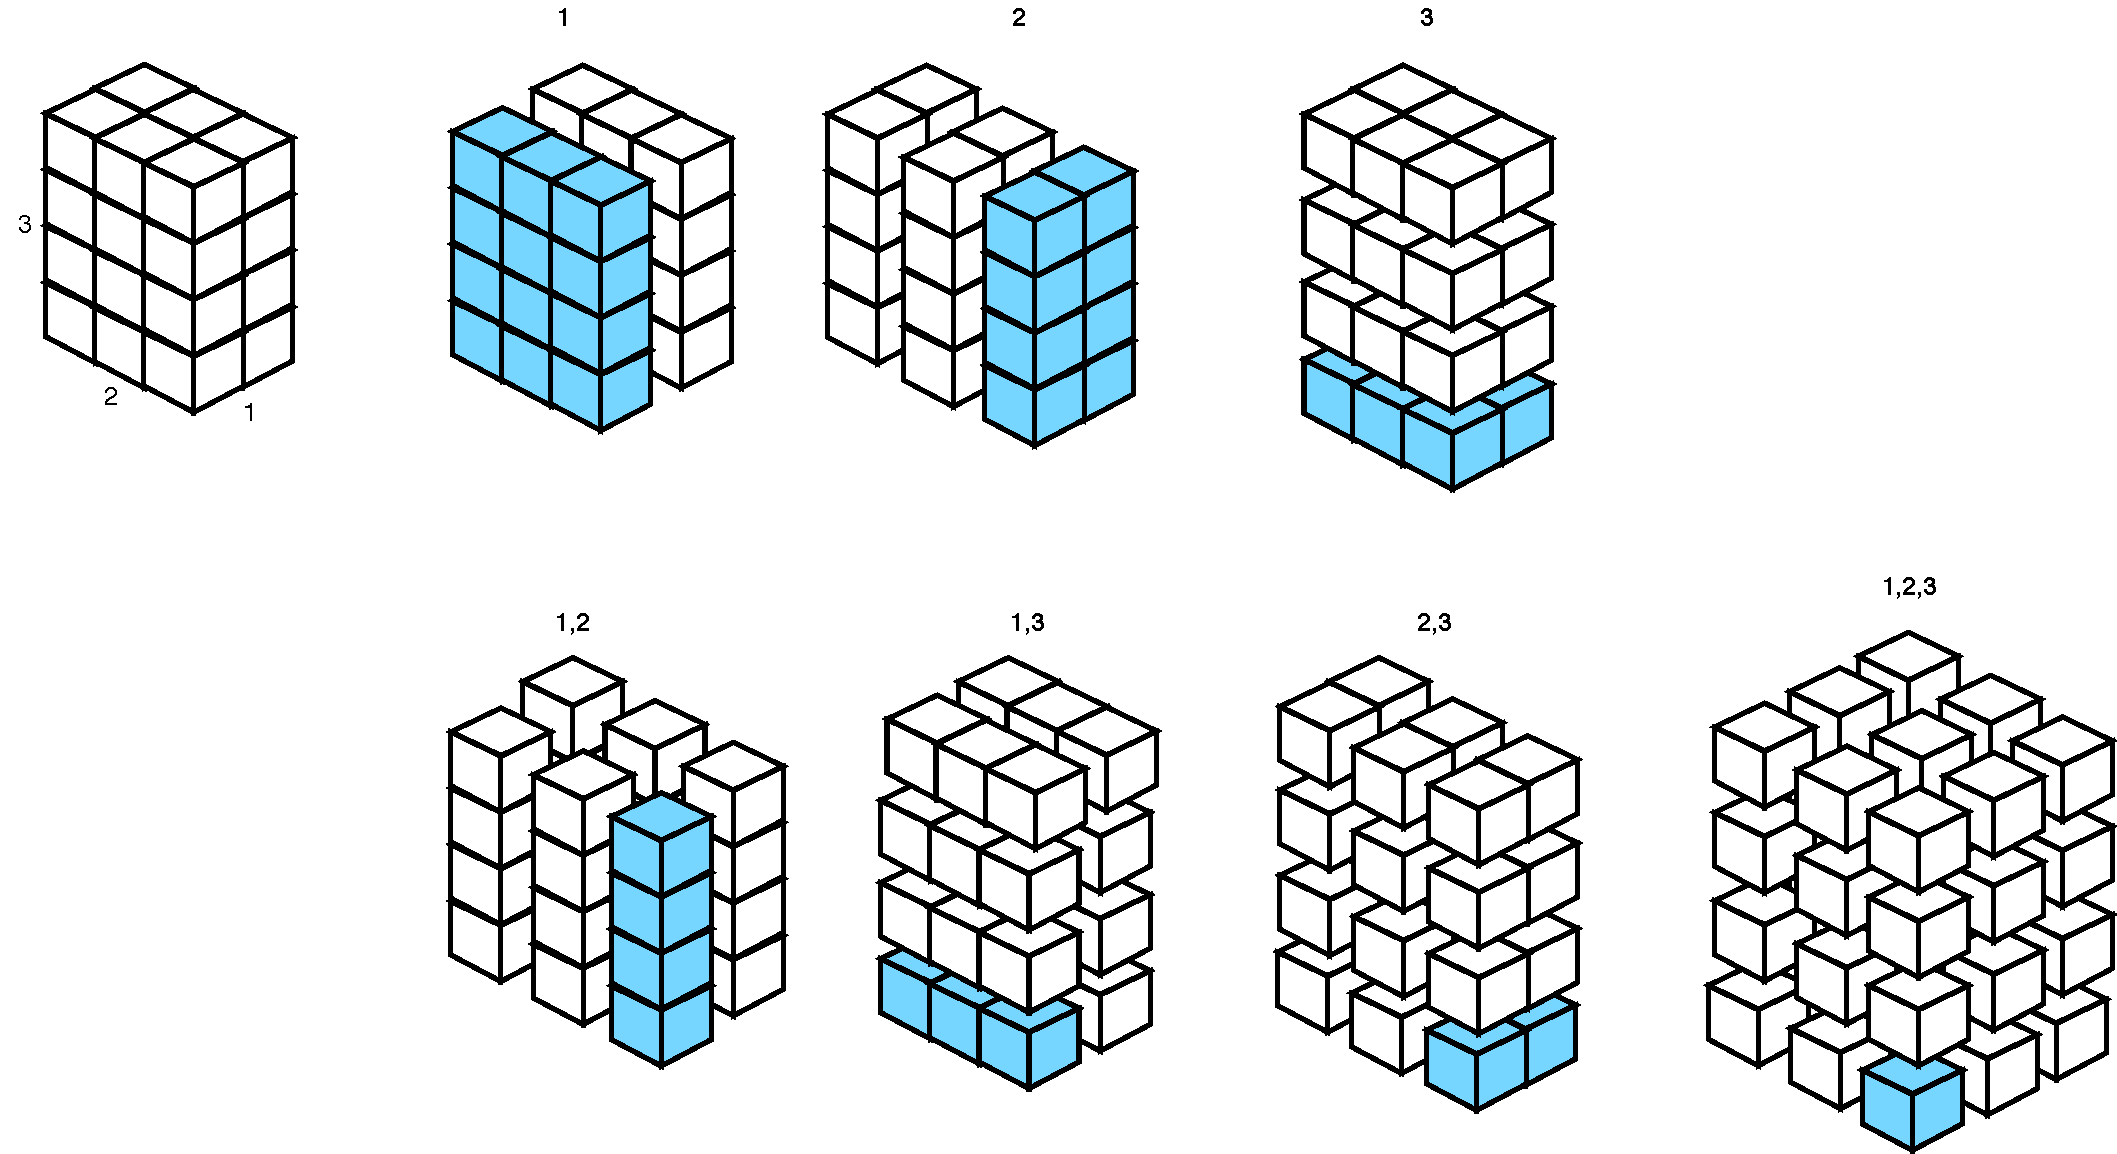
\includegraphics[width= 0.5 \textwidth]{split-array}
  \caption{The seven ways to split up a 3d array.  Original array shown at top left.  Blue indicates a single piece of the output.}
  \label{fig:split-array}
\end{figure}

A special case of operating on arrays corresponds to the {\tt mapply} function of base R.  The plyr equivalents are named {\tt maply}, {\tt mdply}, {\tt mlply} and {\tt m\_ply}.  These default to working on the first dimension (i.e. row-wise) and automatically splat the function so that function is called not with a single list as input, but each column is passed as a separate argument to the function.  Compared to using {\tt mapply}, for the {\tt m*ply} functions you will need to {\tt cbind} the columns together first.  This will ensure that each argument has the same length, and allows the {\tt m*ply} functions to have the same argument order as all the other 

Can pass data frame if want to treat as 2d structure.  

\subsubsection{In: data frame ({\tt d*ply})}

When operating on a data frame, you usually want to split it up into groups based on combinations variables in the data set.  For {\tt d*ply} you specify   which variables (or functions of variables) to use.  These variables are specified in a special way to highlight that they are computed first from the data frame, then the global environment (in which case it's your responsibility to ensure that their length is equal to the number of rows in the data frame).  

\begin{itemize}
  \item The interaction of multiple variables are taken: {\tt .(a, b, c)}
  \item Functions of variables: {\tt .(round(a))}, {\tt .(a * b)}
  \item Variables in the global environment {\tt .(anothervar)}
\end{itemize}

\subsection{Output}
\label{sec:output}

The output type defines how the pieces will be joined back together again, and how they will be labelled.  The labels are particularly important to allow you to match up the input with the output.

The input and output types are the same, except there is an additional output option, which discard the output.  This is useful for functions with side effects that make changes outside of R

The output type also places some restrictions on what type of results the processing function should return.  Generally, the processing function should return the same type of data as the eventual output, (i.e.\ vectors, matrices and arrays for {\tt *aply} and data frames for {\tt *dply}) but some other formats are accepted for convenience and are described below.  

% For any type, if the processing function returns {\tt NULL}, that slice will not be included in the output.

\subsubsection{Out: array ({\tt *aply})}

With array output the dimensionality is determined by the input splits.  A list will produce a single dimension, a data frame will have a dimension for each variable split on, and a array will have a dimension for each dimension that it was split on.  The processing function should return an atomic (i.e.\ {\tt is.atomic(x) == TRUE}) of array of fixed size/shape, or a list.  If atomic, the extra dimensions will added perpendicular to the original dimensions.  If a list, the output will be a list with dimensions.  

Some examples should make this easier to understand:


\begin{figure}[htbp]
  \centering
    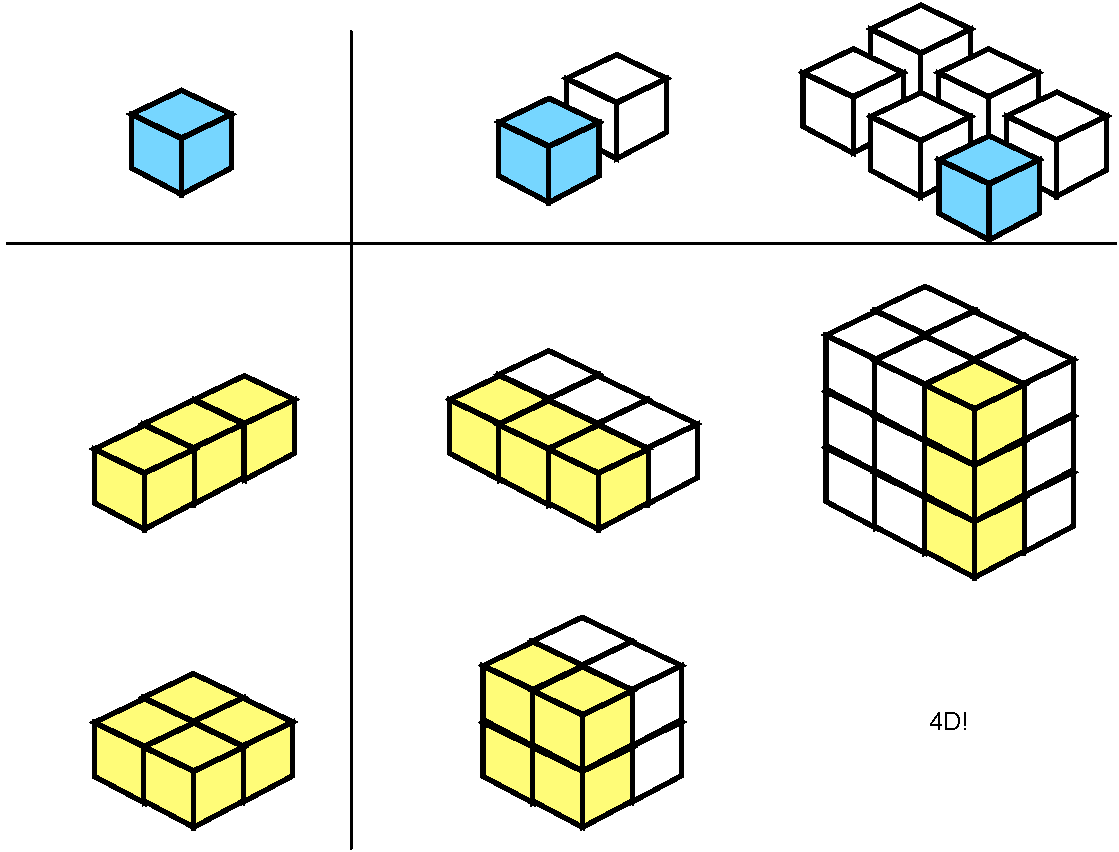
\includegraphics[width= 0.5 \textwidth]{function-1d}
  \caption{Results from outputs of various dimensionalty from a single value, shown top left.  Columns indicate input and rows output from function.  The array in the bottom-right cell is 4d and so is not shown.}
  \label{fig:function-1d}
\end{figure}

\begin{figure}[htbp]
  \centering
    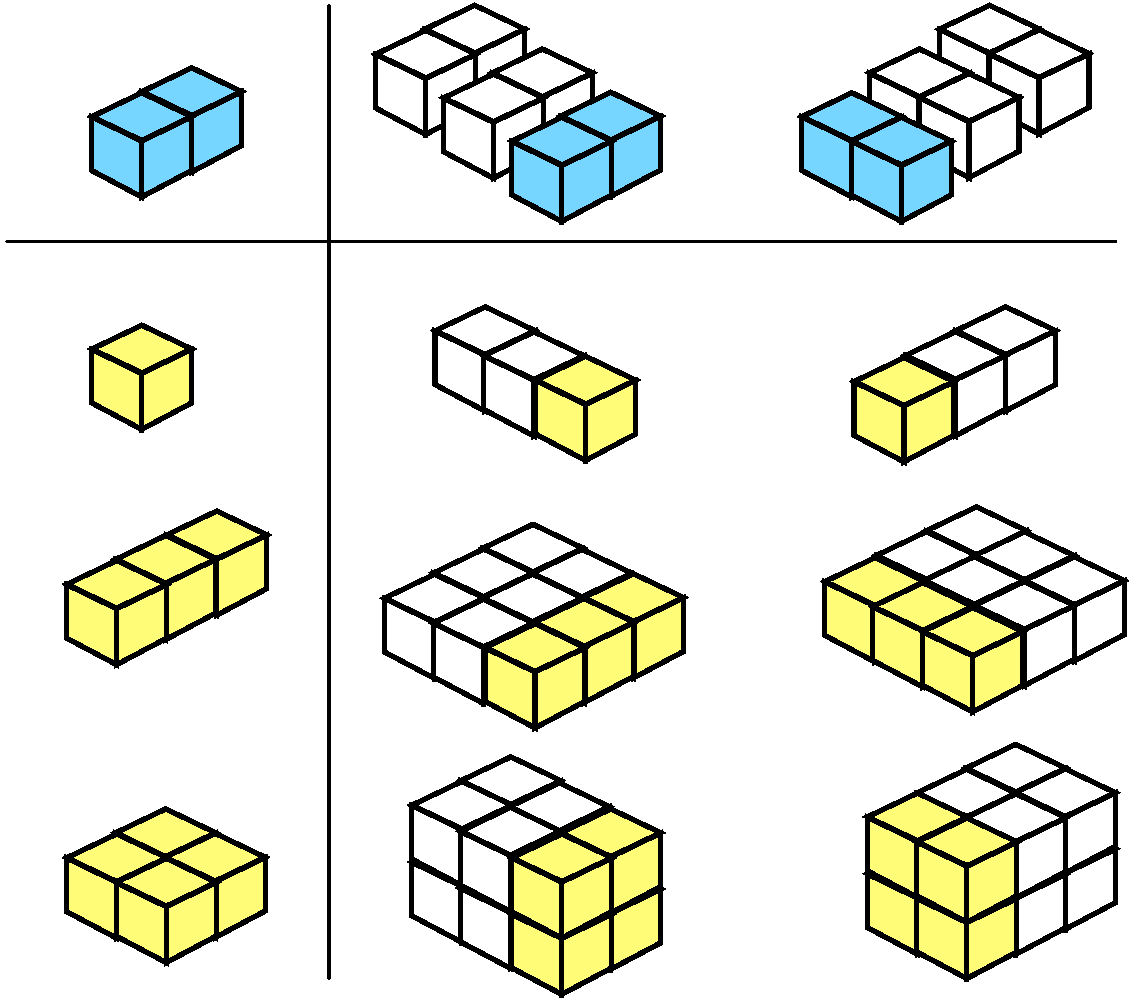
\includegraphics[width= 0.5 \textwidth]{function-2d}
  \caption{Results from outputs of various dimensionalty from a 1d vector, shown top left.  Columns indicate input and rows output from function.}
  \label{fig:function-2d}
\end{figure}


The dimnames of the array will be the same as the input, if an array, or the extracted from the subsets if a data frame.

If there are no results, {\tt adply} will return a logical vector of length 0.

\subsubsection{Out: data frames ({\tt *dply})}

The processing functions should either return a data.frame, or a (named) atomic vector of fixed length, which will form the columns of the output.

If there are no results, {\tt *dply} will return an empty data frame.

The output data frame will be supplemented with columns that identify the subset of the original dataset that each piece was computed from.  These columns make it easier to merge the old and new data.  If the input was a data frame, this will be the values of the splitting variables.  If the input was an array, this will be the dimension names.

\subsubsection{Out: list ({\tt *lply})}

This is the simplest output format, where each processed piece is joined together in a list.  The list also stores the labels associated with each pieces, so that if you use {\tt ldply} or {\tt laply} to further process the list the labels will appear as if you had used {\tt aaply}, {\tt adply}, {\tt daply} or {\tt ddply} directly.  {\tt llply} is convenient for calculating complex objects once (e.g.\ models), from which pieces of interest are later extracted into arrays and data frames.

There are no restrictions on the output of the processing function.  If there are no results, {\tt *lply} will return a list of length 0.

\subsection{Out: nothing ({\tt *\_ply})}

Sometimes you are operating on a list purely for the side effects (e.g. plots, caching, output to screen/file).  This is a little more efficient than abandoning the output of {\tt *lply} because it doesn't store the intermediate results.

\section{Helpers}
\label{sec:helpers}

The {\tt plyr} package also provides a number of helper function which take a function (or functions) as input and return a modified function as output.  

\begin{itemize}
  \item {\tt splat} converts a function to use.  This is useful when you want to pass a function a row of data frame or array, and don't want to manually pull it apart in your function.  For example:
  
  \begin{verbatim}
    hp_per_cyl <- function(hp, cyl, ...) hp / cyl
    splat(hp_per_cyl)(mtcars[1,])
    splat(hp_per_cyl)(mtcars)
  \end{verbatim} 
  
  Generally, splatted functions should have {\tt ...} as an argument, so you only need to specify the variables that you are interested in.  For more information on how splat works, see {\tt do.call}.  
  
  {\tt splat} is applied to functions used in {\tt m*ply} by default.

  \item {\tt each} takes a list of functions and produces a function that runs  each function on the inputs and returns a named vector of outputs.   For example, {\tt each(min, max)} is short hand for {\tt function(x) c(min = min(x), max = max(x))}.  Using each with a single function is useful if you want a named vector as output.

  \item {\tt colwise} converts a function that works on vectors, to one that operates column-wise of data frame, returning a data fram.  For example, {\tt colwise(median)} is a function that computes the median of each column of a data.frame.  
  
  The optional {\tt .if} argument specialises the function to only run on certain types of vector, e.g.\ {\tt .if = is.factor} or {\tt .if = is.numeric}.  These two restrictions are provided in the premade {\tt calcolwise} and {\tt numcolwise}.  
  
  \item {\tt failwith} sets a default value to return if the function throws an error.  For example, {\tt failwith(NA, f)} will return an {\tt NA} whenever {\tt f} throws an error.  
  
  The optional {\tt quiet} argument suppresses any notice of the error when it is {\tt TRUE}.

  \item {\tt e2f} converts an expression to a function.  This allows you to imitate {\tt replicate}.

\end{itemize}

Each plyr function also has a {\tt .progress} argument which allows you to monitor the progress of long running operations.  There are four difference progress bars:

\begin{itemize}
  \item {\tt "none"}, the default.  No progress bar is displayed.
  \item {\tt "text"} provides a textual progress bar which.
  \item {\tt "win"} and {\tt "tk"} provide graphical progress bars for Windows and systems with the tcl/tk package loaded.
\end{itemize}

The progress bars assume that processing each piece takes the same amount of time, so will not be 100\% accurate.

\section{Strategy}
\label{sec:strategy}



\begin{enumerate}
  \item Extract a subset of the data for which it is easy to solve the problem
  \item Solve the problem by hand, checking as you go
  \item Write a function that encapsulates the solution
  \item Use the appropriate ply function to split up the original data, apply the function and join the pieces back together.
  
\end{enumerate}

The following two case studies illustrate these techniques for a range of problems related to a data frame storing the batting records for long-term baseball players, and a 3d array representing space and time values of ozone.

\subsection{Case study: baseball data}

The {\tt baseball} data set contains the batting records for all professional US players with 15 or more years of data.  The complete list of variables are described fully {\tt ?baseball}, but for this example we will focus on just four: {\tt id}, which identifies the player, {\tt year} the year of the record and {\tt rbi} the number of runs that the player made in the season, and {\tt} at bat, the number of times the player had an opportunity to hit the ball.

(This is a rather crude analysis, as it doesn't take into account the people that might already be on the other plates)

What we'll explore is the performance of a batter over his career.  To get started, we need to calculate the careeryear, i.e. the number of years since the player started playing.  This is easy to do if we have a single player:

\begin{verbatim}
baberuth <- subset(baseball, id == "ruthba01")
baberuth$cyear <- baberuth$year - min(baberuth$year) + 1
\end{verbatim}

To do this for all players, we first make a function:

\begin{verbatim}
calculate_cyear <- function(df) {
  transform(df, 
    cyear = year - min(year),
    cpercent = (year - min(year)) / (max(year) - min(year))
  )
}
\end{verbatim}

\noindent and then split up the whole data frame into people, run the function on each piece and join them back together into a data frame:

% qplot(ab, data=baseball, geom="histogram", binwidth=10)
% qplot(ab, data=subset(baseball, ab < 100), geom="histogram", binwidth=5)

\begin{verbatim}
baseball <- ddply(baseball, .(id), calculate_cyear)
baseball <- subset(baseball, ab >= 25)
\end{verbatim}

% qplot(cyear, rbi / ab, data=baseball, group=id, geom="line", colour=I(alpha("black", 1/20)))

To summarise the pattern across all players, we first need to figure out what the common patterns are.  A time series plot of rbi/ab, runs per bat, is a good place to start.  We do this for Babe Ruth, as shown in Figure~\ref{fig:baberuth}, then write a function to do it for any player (taking care to ensure common scale limits) and then use {\tt d\_ply} to save a plot for every player to a pdf.  We use two tricks here: {\tt reorder} to sort the players in order of average rbi / ab, and {\tt failwith} to ensure that even if a single plot doesn't work we will still get output for the others.

\begin{figure}[htbp]
  \centering
    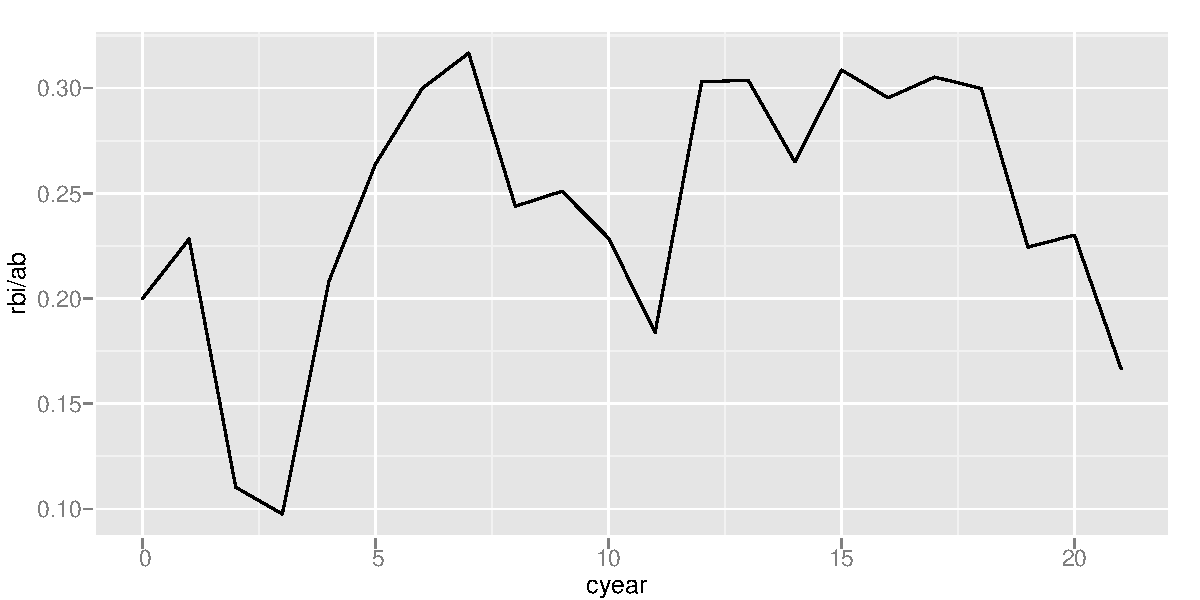
\includegraphics[width=3in]{baberuth}
  \caption{Runs per bat for Babe Ruth.}
  \label{fig:baberuth}
\end{figure}

\begin{verbatim}
qplot(cyear, rbi / ab, data=baberuth, geom="line")  

xlim <- range(baseball$cyear, na.rm=TRUE)
ylim <- range(baseball$rbi / baseball$ab, na.rm=TRUE)
plotpattern <- function(df) {
  print(qplot(cyear, rbi / ab, data = df, geom="line", xlim = xlim, ylim = ylim ))
}

pdf("paths.pdf", width=8, height=4)
d_ply(baseball, .(reorder(id, rbi / ab)), failwith(NA, plotpattern))
dev.off()
\end{verbatim}

Flicking through the 1145 plots reveals that there doesn't seem to be much of a common pattern, although many players do seem to have a roughly linear trend with quite a bit of noise.  We'll start by fitting a linear model to each player and then exploring the results.  This time we'll skip doing it by hand and go directly to the function.

\begin{verbatim}
model <- function(df) {
  lm(rbi / ab ~ cyear, data=df)
}
model(baberuth)
models <- dlply(baseball, .(id), model)
\end{verbatim}

Now we have a list of 1145 models, one for each player.  To do something interesting with these, we need to extract some summary statistics.  We'll extract the coefficients of the model (the slope and intercept), and a measure of model fit so we can ensure we're not drawing conclusions based on models that fit the data very poorly, the R-squared.  The first few rows of {\tt coef} are shown in Table~\ref{tbl:coef}.

\begin{verbatim}
rsq <- function(x) summary(x)$r.squared
coef <- ldply(models, function(x) c(coef(x), rsq(x)))
names(coef) <- c("id", "intercept", "slope", "rsquare")
\end{verbatim}

\begin{table}[ht]
  \centering
  \begin{tabular}{lrrr}
    \hline
    id & intercept & slope & rsquare \\
    \hline
    aaronha01 & 0.18 & 0.00 & 0.00 \\
    abernte02 & 0.00 &  & 0.00 \\
    adairje01 & 0.09 & $-$0.00 & 0.01 \\
    adamsba01 & 0.06 & 0.00 & 0.03 \\
    adamsbo03 & 0.09 & $-$0.00 & 0.11 \\
    adcocjo01 & 0.15 & 0.00 & 0.23 \\
    \hline
  \end{tabular}
  \caption{The first few rows of the {\tt coef} data frame.  Note that the player ids from the original data have been preserved}
  \label{tbl:coef}
\end{table}

Figure~\ref{fig:models-hist} displays the distribution of r-squared across the models.  The models generally do a very bad job of fitting the data!  
Figure~\ref{fig:models} summarises these bad models.  These plots show a negative correlation between slope and intercept, and the particularly bad models have estimates for both values close to 0.  Reassuringly, there are no players in the bottom left quadrant with both negative slope and intercept.

% qplot(rsquare, data=coef, geom="histogram", binwidth=0.01)
% ggsave(file = "models-hist.pdf", width=12, height=4)
\begin{figure}[htbp]
  \centering
    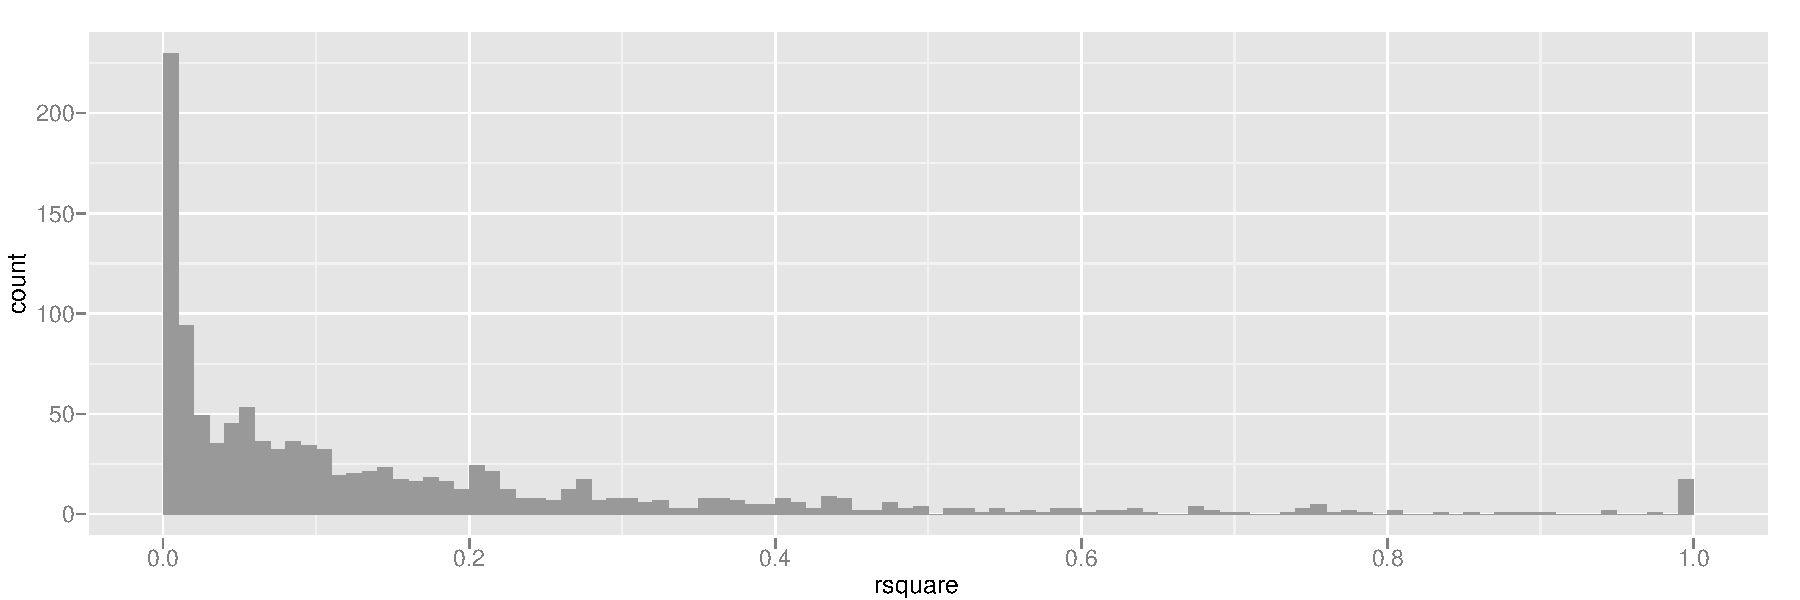
\includegraphics[width=6in]{models-hist}
  \caption{Histogram of model r-squared with bin width of 0.05.  Most models fit very poorly!  The spike of models with a r-squared of 1 are players with only two data points, found by inspecting {\tt ldply(models[coef\$rsquare == 1], "[[", "model")}}
  \label{fig:models-hist}
\end{figure}

% ggplot(coef, aes(slope, intercept)) + 
%   geom_point(aes(size = rsquare)) +
%   geom_vline(size=0.5, colour="grey50") + 
%   geom_hline(size = 0.5, colour="grey50") + 
%   scale_area()
% ggsave(file = "models.pdf", width=6, height=6)
% last_plot() + xlim(-0.01, 0.01) + ylim(-0.1, 0.25)
% ggsave(file = "models-zoom.pdf", width=6, height=6)
\begin{figure}[htbp]
  \centering
    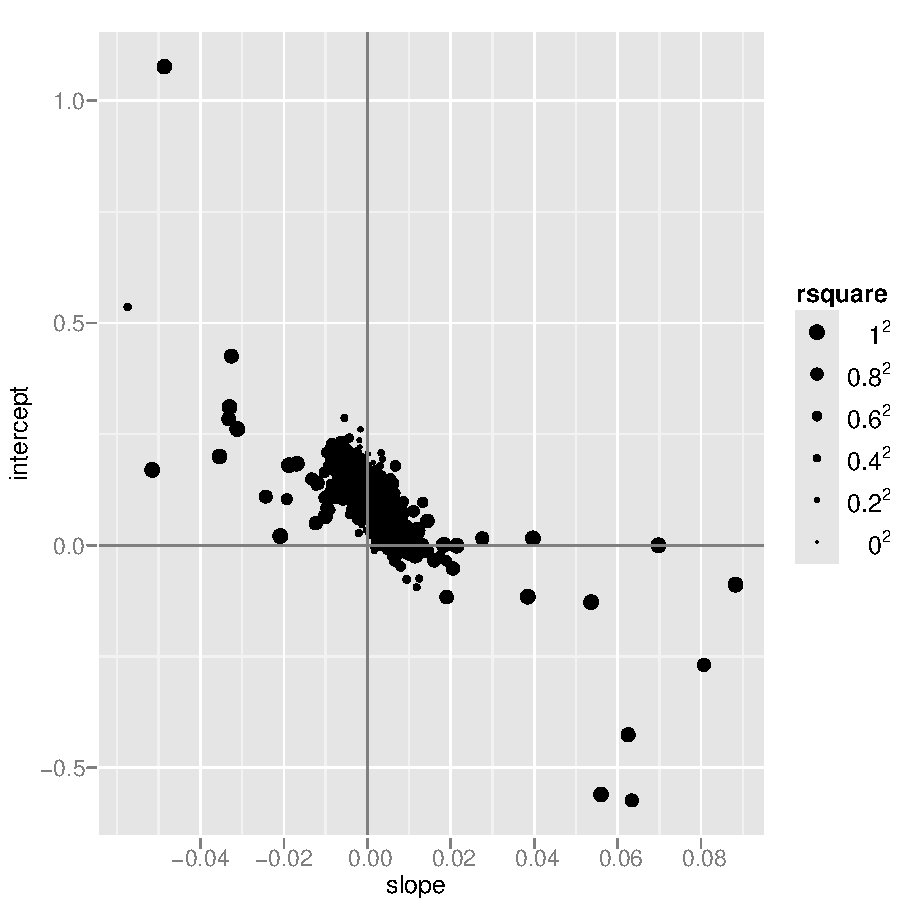
\includegraphics[width=3in]{models}
    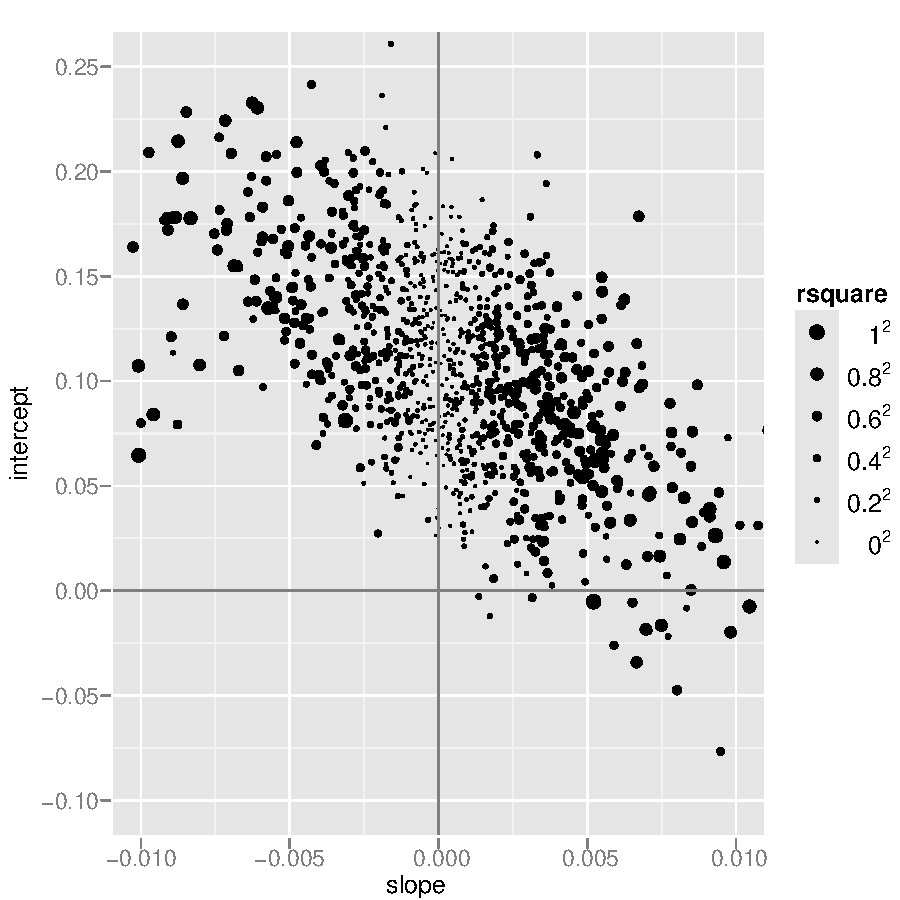
\includegraphics[width=3in]{models-zoom}
  \caption{A scatterplot of model intercept and slope, with one point for each model (player).  The size of the points is proportion to the R-square of the model. Vertical and horizontal lines emphasis the x and y origins. }
  \label{fig:models}
\end{figure}

This concludes the baseball player case study, which used used {\tt ddply}, {\tt d\_ply}, {\tt dlply} and {\tt ldply}.  Our statistical analysis was not very sophisticated, but the tools of {\tt plyr} made it very easy to work at the player level, and then combine results into a single summary.  

\subsection{Case study: spatio-temporal ozone distribution}

Standardisation/smoothing.  \citep{hobbs:2007}

\begin{figure}[htbp]
  \centering
    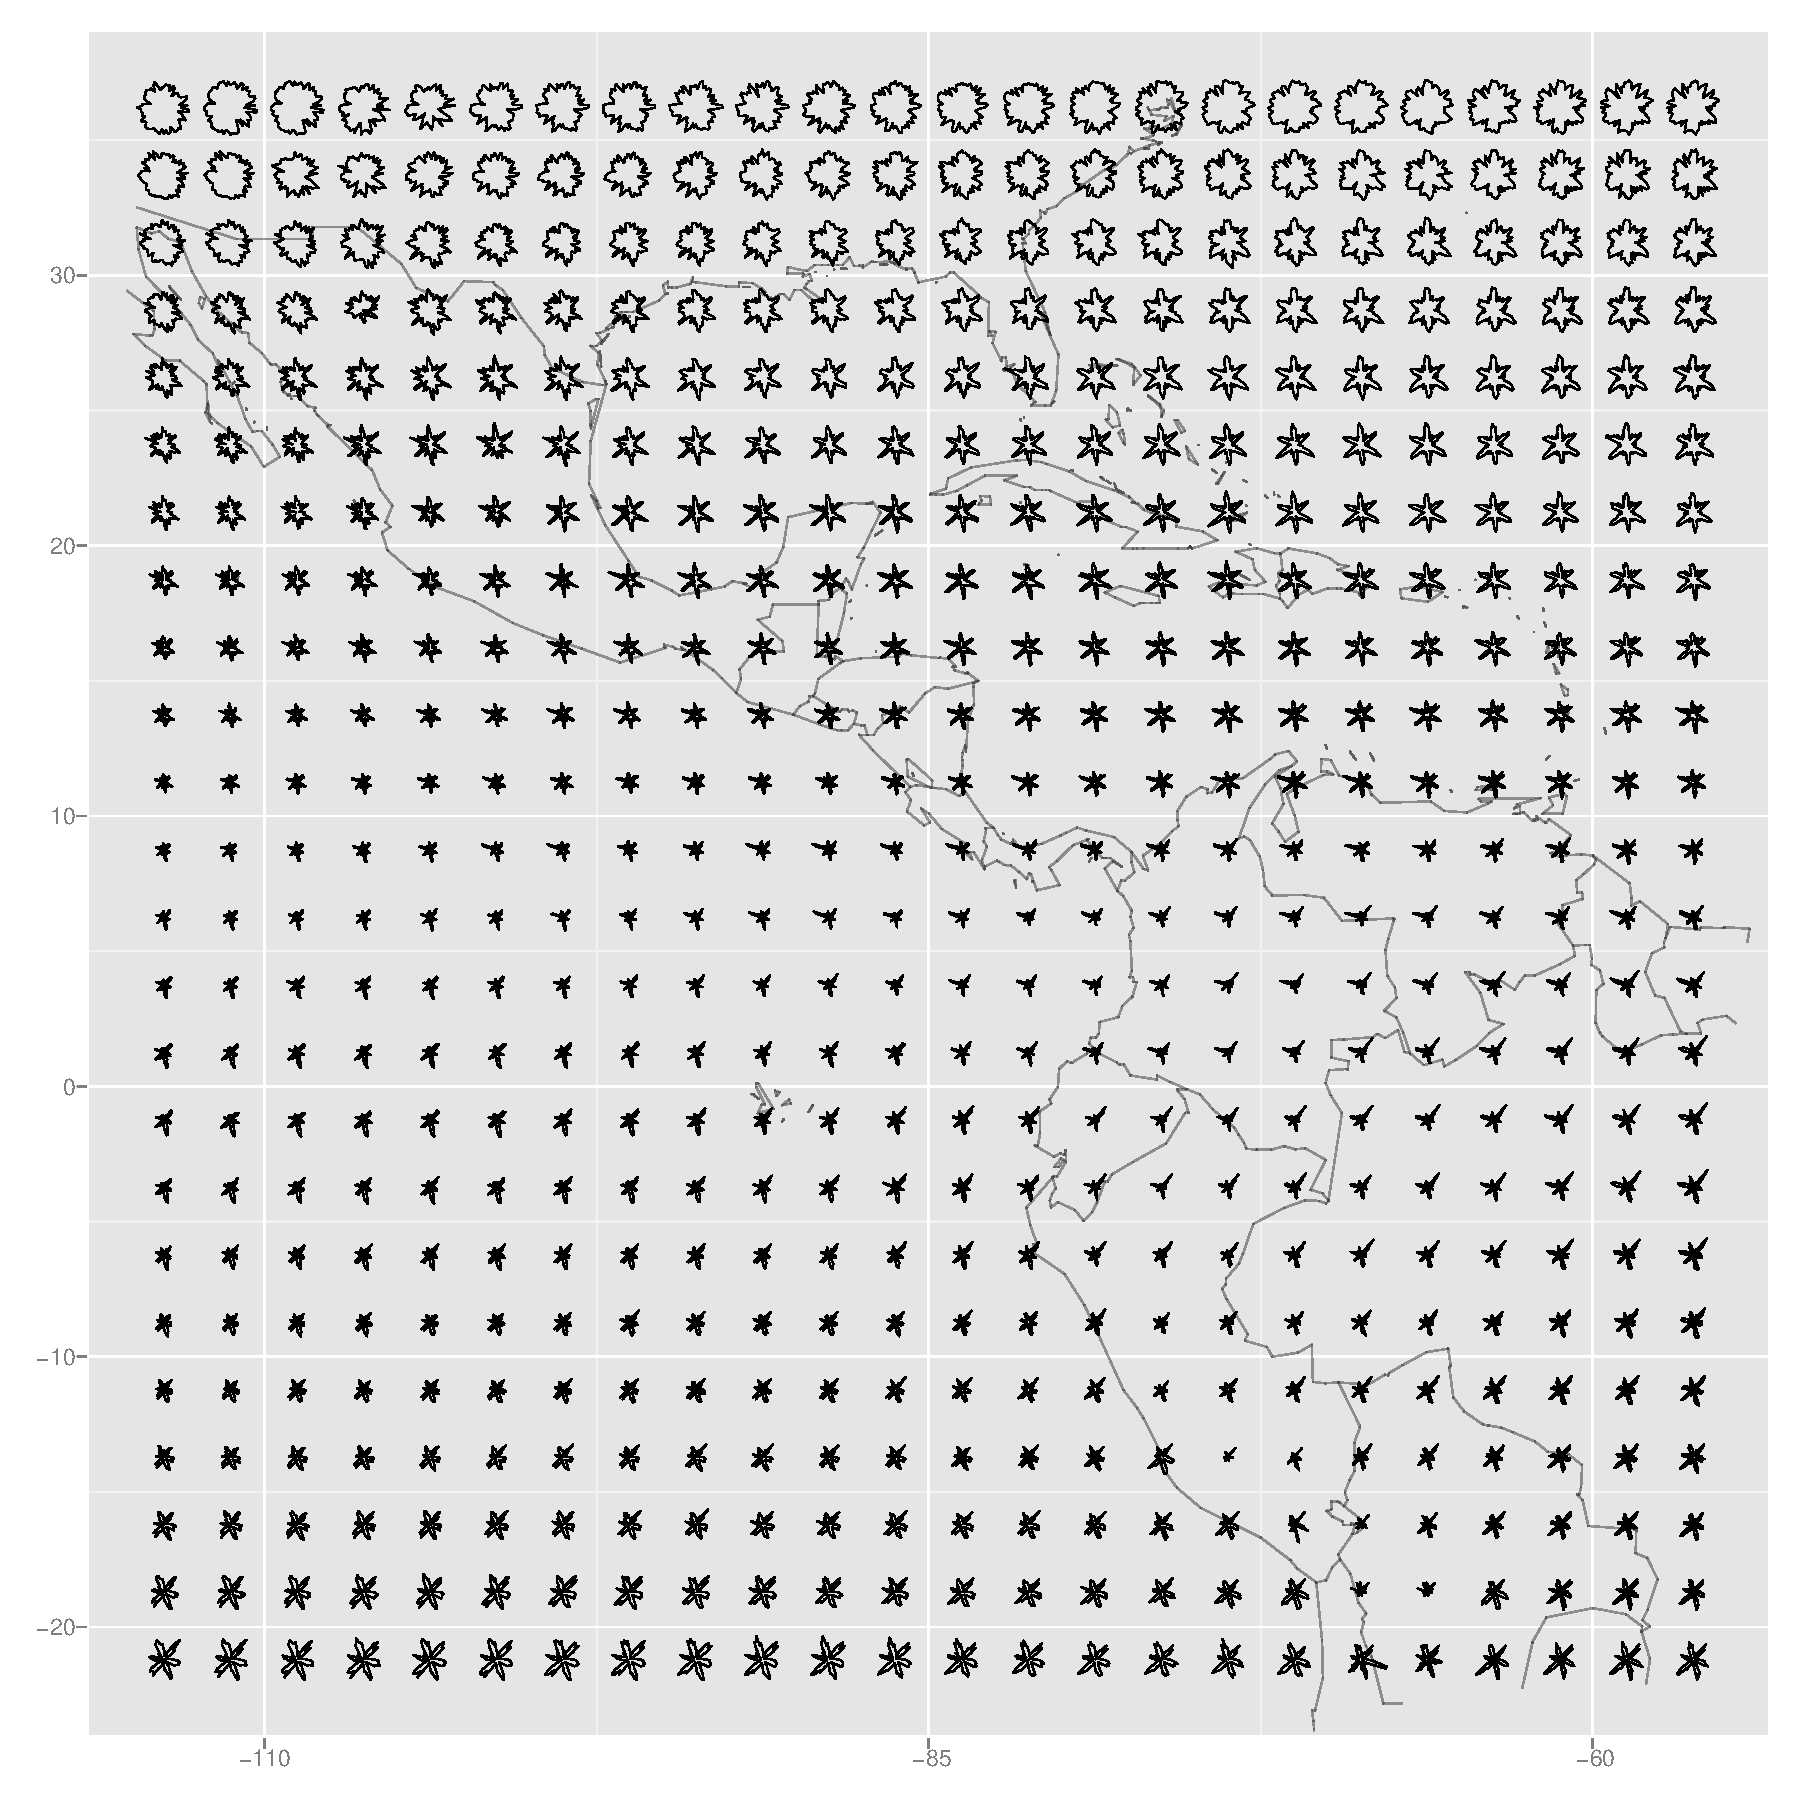
\includegraphics[width=4in]{ozone-glyph}
  \caption{Star glyphs showing variation in ozone over time at each spatial location.}
  \label{fig:ozone-glyph}
\end{figure}

For many other types of operations, it is useful to convert this array structure to a data frame.  The {\tt melt} function in the {\tt reshape} package is one way to do that which preserves the dimension labels as much as possible.

\section{Equivalence to existing R functions}
\label{sec:equiv}

Table~\ref{tbl:equiv} describes the equivalent between functions in base R and 
the functions provided by {\tt plyr}.  The built in R functions focus mainly on arrays and lists, not data frames, and most provide an argument to determine whether an array or list should be returned.  The syntax is also less consistent than plyr, for example, {\tt mapply} takes a function as the first argument rather than the input data.  Compared to {\tt apply}, {\tt aaply} returns the dimensions in a different order so as to be idempotent - i.e.\ {\tt apply(x, a, function(x) x) == x} for all {\tt a}. 

Avoid any ambiguity about what you'll get back from one of these functions. This replaces the {\tt simplify} argument that many of the {\tt apply} functions in base R has, and means that you can depend on the output of each function being a given type (which makes programming with the results easier).


\begin{table}[htpb]
  \begin{center}
  \begin{tabular}{llll}
    base & from & to & plyr \\
    \hline
    apply     & a & a   & aaply \\
    lapply    & l & l   & llply \\
    sapply    & l & a   & laply \\
    mapply    & a & a/l & maply / mlply \\
    by        & d & l   & dlply \\
    aggregate & d & d   & ddply + colwise \\
  \end{tabular}
  \end{center}
  \caption{Mapping between apply functions and plyr functions.}
  \label{tbl:equiv}
\end{table}

Related functions {\tt tapply}, {\tt ave} and {\tt sweep} have no corresponding function in {\tt plyr}, and still remain useful. {\tt merge} is also for combining summaries with the original data.  The cast function in the reshape package \citep{reshape} is closely related to {\tt aaply}.

There are a number of other resources that also attempt to simplify this class of problems:

\begin{itemize}
  \item The {\tt doBy} package
  \item The {\tt gdata} package
  \item The {\tt scope} package
  \item Data manipulation in R, by Phil Spector
  \item Chapters in MASS, R intro?
  
\end{itemize}

\section{Future plans}
\label{sec:future}

If slow, might want to look at the profr package to speed up.  

However, it is my aim to eventually implement these functions in C for maximum speed and memory efficiency, so that they are competitive with the built in operations.  I also plan to investigate a connection to the {\tt papply} function to allow for easy parallelisation across multiple instances of R (particularly for multi-core machines).

multir

\bibliography{/Users/hadley/documents/phd/references}
\end{document}
